\section{LingBot-World-Infinity}\label{sec:method}

As shown in \cref{fig:model_pipeline}, {\method} takes an initial frame and interacts with a stream of user inputs to autoregressively generate an infinite world that extends endlessly in real time and remains drift-free over arbitrarily long horizons.
%
To this end, we first formalize the interactive world simulator as a causal generative process (\cref{sec:formulation}). 
%
Building on this formulation, we adopt a two-stage strategy to train {\method}: a \textbf{pre-training} stage that learns a causal, action-conditioned world model~(\cref{sec:pretraining}), and a \textbf{post-training} stage that distills the model into a real-time generator and suppresses long-horizon drift~(\cref{sec:posttraining}).

\begin{figure*}[t]
\centering
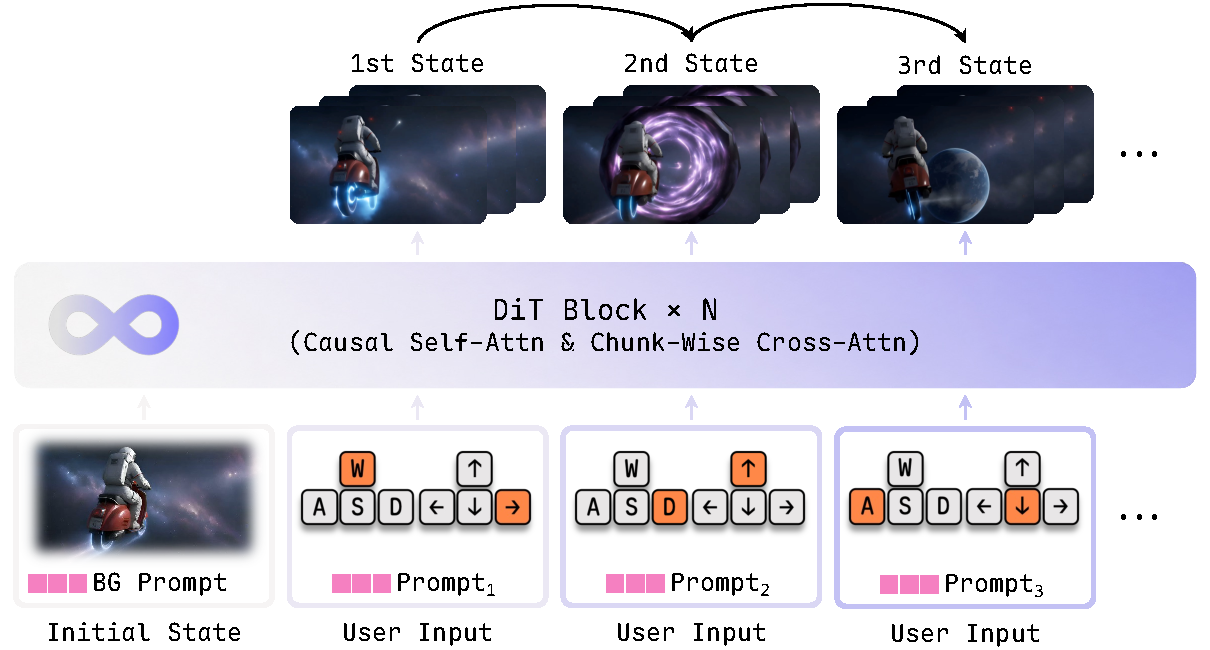
\includegraphics[width=\linewidth]{figures/pretrain/pretrain.pdf}
\caption{\textbf{Overview of \method Pipeline.} 
An interactive world simulator is implemented as a causal video model.
Our Infinity World is initialized from an initial image and its background description.
The future world states are then autoregressively generated, conditioned on the historical context and user inputs (camera poses and prompts).}
\label{fig:model_pipeline}
\end{figure*}

\subsection{Formulation}
\label{sec:formulation}
%
\begin{quote}
\itshape ``The cause must be prior to the effect.'' \par
\normalfont\hfill --- David Hume, \emph{A Treatise of Human Nature}~\cite{hume2000treatise}
\end{quote}
The first principle of causal reasoning is that an effect never precedes its cause: the future is shaped by the past, never the reverse.
%
We follow this principle to introduce {\method}, an interactive world simulator where each state is generated from past visual observations and the current user input.
%
We therefore cast world simulation as a causal generative process along the time axis. 
Let $\mathcal{V} = \{x_1, x_2, \dots, x_T\}$ denote a sequence of video frames, where $x_t \in \mathbb{R}^{H \times W \times C}$ represents the visual state at time step $t$, and let $\mathcal{A} = \{a_1, a_2, \dots, a_T\}$ denote the corresponding sequence of user inputs (including control signals and action prompts).
Under the causal assumption, each state depends solely on its historical context $(x_{<t}, a_{\le t})$, yielding the factorization:
\begin{equation}
\label{equ:causal_factorization}
    p_\theta(x_{1:T} \mid a_{1:T}) = \prod_{t} p_\theta\!\left(x_t \mid x_{<t}, a_{\le t}\right)
\end{equation}
where $\theta$ parameterizes the world transitions and dynamics that {\method} learns by maximizing this causal likelihood over large-scale video data.
%
In this work, we enforce causality natively throughout training, as detailed in the following two stages.

\subsection{Pre-Training: Causal World Model}
\label{sec:pretraining}
%
In the pre-training stage, we train a causal world model that generates a boundless, action-controllable video world with high visual fidelity.
%
As illustrated in \cref{fig:attn_mask}, we support two forms of user input, camera poses and prompts, as actions, enabling rich interactive control.
%
Moreover, we propose \textbf{Mixture of Bidirectional and Autoregressive Attention Mask}, a causal self-attention mask where a bidirectional component is appended to the teacher forcing~\cite{williams1989learning} mask, enabling autoregressive generation while preserving the fidelity of the base generator.
%
We also design a causal cross-attention mask for leak-free conditioning and flexible interaction.

\begin{figure*}[t]
\centering
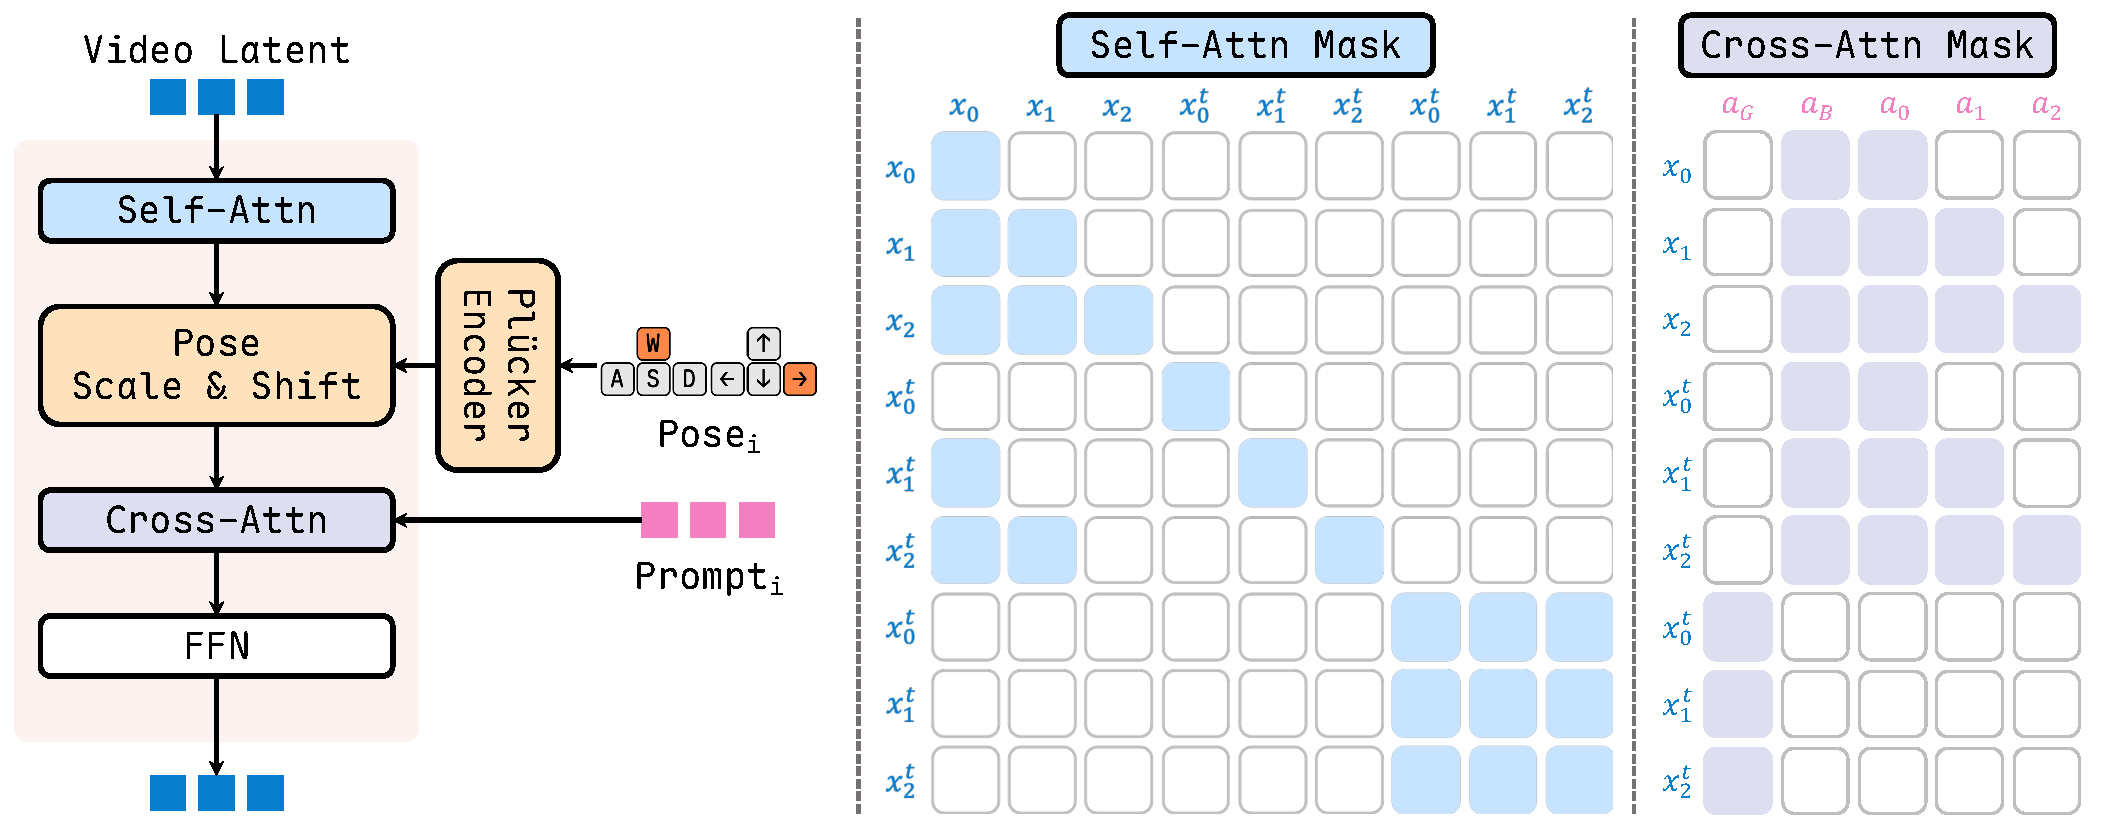
\includegraphics[width=\linewidth]{figures/pretrain/pretrain_mask.pdf}
\caption{\textbf{Overview of \method DiT Block and MoBA Attention Mask.} 
The action comprises camera poses and chunk-wise prompts, injected into the DiT block to enable user interaction.
For self-attention, a bidirectional block is appended to teacher forcing mask, enabling autoregressive generation while preserving visual fidelity.
For cross-attention, the autoregressive component attends to a background prompt and chunk-wise prompts of lower-triangular pattern to prevent access to future information, while the bidirectional component attends to a global prompt.}
\label{fig:attn_mask}
\end{figure*}

\noindent\textbf{Action Representation.}
%
In {\method}, the action comprises two forms of user input: camera poses and textual prompts.
%
For camera control, we represent camera pose using {Pl\"ucker embeddings}~\cite{he2024cameractrl,he2025cameractrl}, which encode the viewing ray of each pixel as six-dimensional coordinates, and utilize an adaptive layer normalization~(AdaLN) mechanism~\cite{xu2019understanding} to incorporate these control signals into the diffusion process without disrupting the pre-trained visual priors.
%
For textual control, we adopt chunk-wise prompts for autoregressive video generation, where each video chunk is assigned its own caption, enabling time-localized semantic control. We detail how these chunk-wise prompts are injected via cross-attention mask below.

\noindent\textbf{Mixture of Bidirectional and Autoregressive~(MoBA) Attention Mask.}
%
With teacher forcing mask, the model predicts the current state from the clean context for autoregressive video generation.
However, we find that the longer the context grows, the more our model learns to rely solely on the context instead of predicting future frames, resulting in overfitting and visual quality degradation.
%
Therefore, we propose MoBA mask, a hybrid attention mechanism, to counter this issue by integrating a bidirectional component into teacher forcing mask.
As illustrated in \cref{fig:attn_mask}, the self-attention MoBA mask starts from teacher forcing, where each noisy frame $x_i^{t}$ (frame $i$ at noise timestep $t$) attends only to itself and its clean context $x_{<i}$.
A bidirectional component with full attention (the bottom-right block of the mask) is then integrated, helping the model adapt to flexible-length video generation and promoting its transition from bidirectional to autoregressive generation. 
It also serves as a regularizer that mitigates the overfitting of pure teacher forcing, thereby avoiding visual quality degradation.
%
To match two components of MoBA, we design a corresponding cross-attention mask. 
For the teacher forcing component, each frame attends to a background prompt $a_{B}$ together with the chunk-wise prompts $a_{\le i}$ of the current and all preceding chunks in a lower-triangular pattern, preventing any future semantics from leaking in. 
For the bidirectional component, which already attends over all frames, we follow standard practice and use a global prompt $a_{G}$ that describes all events throughout the video.

\noindent\textbf{Training objective.}
We optimize {\method} with a conditional flow-matching objective. 
For each frame $i$, we construct a noisy latent $x_i^{t} = (1-t)\,x_i + t\,\epsilon$ with $t \sim \mathcal{U}(0,1)$ and $\epsilon \sim \mathcal{N}(0,\mathbf{I})$, and train the network $v_\theta$ to predict the flow velocity conditioned on the clean context $x_{<i}$, the camera pose $p_{\le i}$, and the prompt $a_{\le i}$:
\begin{equation}
\label{equ:pretrain_loss}
    \Loss_{\text{fm}} = \E_{x,\, i,\, t,\, \epsilon}
    \left\| v_\theta\!\left(x_i^{t},\, t \mid x_{<i},\, p_{\le i},\, a_{\le i}\right) - (\epsilon - x_i) \right\|^2,
\end{equation}
where $p_{\le i}$ and $a_{\le i}$ denote the camera poses and prompts up to the current chunk, and the target velocity $\epsilon - x_i$ follows the rectified-flow interpolation.

\subsection{Post-Training: Few-Step Distillation}
\label{sec:posttraining}
%
In the post-training stage, we compress the multi-step pre-trained causal diffusion world model into a few-step generator suitable for real-time interaction, while mitigating the error accumulation that arises over long autoregressive rollouts.
%
To this end, we combine \emph{consistency distillation}~\cite{song2023consistency} to reduce the number of denoising steps with \emph{distribution matching distillation} (DMD)~\cite{yin2024dmd} to improve fidelity and suppress rollout drift.

%
\noindent\textbf{Consistency Distillation.}
Although the pre-trained teacher produces high-quality frames, generating each frame requires many denoising steps, which is prohibitively expensive for interactive use.
%
We therefore distill the teacher into a consistency model~\cite{song2023consistency, lin2025apt2, zheng2026rcm, zhu2026causal} $G_\theta$, which predicts a trajectory-invariant target from an intermediate noisy latent.
%
In particular, latent states lying on the same teacher probability-flow ODE (PF-ODE) trajectory should map to identical predictions under $G_\theta$.
%
Let $x_i^t$ denote the latent state of frame $i$ at diffusion time $t$, and let $\tilde{x}_i^{\,t-\Delta t}$ denote the latent obtained by integrating the teacher PF-ODE from $(x_i^t, t)$ to time $t-\Delta t$, where $\Delta t > 0$.
%
Under the causal conditioning $c = (x_{<i},\, p_{\le i},\, a_{\le i}),$ we enforce local consistency between adjacent points on the same teacher trajectory by minimizing
\begin{equation}
\label{equ:cd_loss}
    \Loss_{\mathrm{CD}}
    =
    \E\!\left[
    d\!\left(
    G_\theta(x_i^t, t \mid c),\;
    G_{\theta^-}(\tilde{x}_i^{\,t-\Delta t}, t-\Delta t \mid c)
    \right)
    \right],
\end{equation}
where $d(\cdot,\cdot)$ is a distance metric and $\theta^-$ denotes an exponential moving average (EMA) of the student parameters $\theta$.
%
The expectation is taken over training samples, diffusion times, and trajectory points induced by the teacher dynamics. 
%
Optimizing~\cref{equ:cd_loss} distills the teacher's multi-step denoising trajectory into a few-step student generator while preserving the action-conditioned dynamics acquired during pre-training.

%
\noindent\textbf{Distribution Matching Distillation.}
%
While consistency distillation substantially reduces the sampling cost, the resulting few-step student generator may still suffer from degraded visual fidelity and compounding drift during long-horizon self-rollout.
%
To further refine the student, we employ distribution matching distillation (DMD)~\cite{yin2024dmd}, which optimizes the generator using the gradient of the KL divergence between the noised student distribution and the noised data distribution.
%
Let $\hat{x}_i$ denote a sample generated by the student, and let $\hat{x}_i^t$ be its noised version obtained by forward diffusion to time $t$.
%
Then the gradient of the objective is given by
\begin{equation}
\label{equ:dmd_loss}
    \nabla_\theta \E\left[D_{\mathrm{KL}}\left(p_{\theta,t} \,\|\, p_{\mathrm{data},t}\right)\right]
    =
    - \E\!\left[
    \left(
    s_{\mathrm{real}}(\hat{x}_i^t, t \mid c)
    -
    s_{\mathrm{fake}}(\hat{x}_i^t, t \mid c)
    \right)
    \frac{\partial \hat{x}_i}{\partial \theta}
    \right],
\end{equation}
%
where the conditioning variable $c = (x_{<i},\, p_{\le i},\, a_{\le i})$ is defined as in~\cref{equ:pretrain_loss}.
%
Here, $s_{\mathrm{real}}$ and $s_{\mathrm{fake}}$ approximate the scores of the noised data distribution and the current noised student distribution, respectively. The expectation is taken over sampled diffusion times and student-generated samples.
%
To improve robustness under deployment-time dynamics, we apply DMD over long self-rollout trajectories rather than only on teacher-forced states~\cite{huang2025self}. 
%
As a result, the student is optimized on the state distribution induced by its own predictions, which reduces accumulated drift over extended autoregressive rollouts.